\section{Ejecución simbólica dinámica}

\section{Contratos Inteligentes y Solidity}
Una blockchain es una base de datos pública, distribuida e inmutable.
En Ethereum cada transacción registrada se refiere a propiedades sobre \textit{direcciones} en la base de datos como el balance de criptomonedas o el estado de un contrato inteligente.
Las transacciones se agrupan en conjuntos de \textit{bloques}, que son la unidad mínima con la que se actualiza el estado de la blockchain.
El historial de bloques agregados a la blockchain (y por ende, las transacciones ejecutadas) es público, y el estado actual de la red puede calcularse a partir de este historial.
Además, los protocolos de consenso utilizados por la red le otorgan garantías de seguridad de que ningún actor podrá forzar el ingreso de información falsificada a ella \cite{protocolos-consenso}.

Como ya dijimos, Ethereum y otras blockchain mantienen un estado de cómputo distribuido, y permiten modificar este estado mediante aplicaciones programadas llamadas contratos inteligentes.
Los contratos inteligentes se corresponden con direcciones dentro de la base de datos que es la blockchain, de la misma forma que se corresponden con direcciones los usuarios tradicionales.
De hecho, en Ethereum los contratos inteligentes y los usuarios tradicionales cuentan con dos tipos de \textit{accounts} distintas.
En el caso de los usuarios humanos el almacenamiento que le corresponde a cada dirección guarda sólo información sobre el balance de criptomonedas, mientras que un contrato inteligente utiliza dos campos adicionales: el \textit{codeHash}, que es utilizado para obener el código ejectuable del contrato y el \textit{storageRoot}, que es necesario para conocer una especie de memoria persistente exclusiva del contrato.
Ambos tipos pueden recibir o enviar mensajes y Ether\footnote{Ether es la criptomoneda utilizada por Ethereum}.
La diferencia en los dos tipos de accounts radica en qué ocurre cuando la account es seleccionada como destinataria de una transferencia de fondos o mensaje.
Mientras que para un usuario humano simplemente se registra el suceso en la blockchain, en el caso de un contrato inteligente, este es el momento en el que el programa se ejecuta, agregando el mensaje que disparó la ejecución al contexto de la misma.
Para poder incluir la transacción en el próximo estado de la blockchain, el minero\footnote{Los ``mineros'' son quienes participan en el protocolo de la blockchain y registran las transacciones publicadas por usuarios en bloques} que registre la transacción debe levantar la EVM y simular la ejecución del contrato para conocer su  resultado y estado final.

La EVM es una máquina de pila casi turing completa.
El lenguaje assembly asociado cuenta con instrucciones para números enteros, instrucciones para control de flujo y otras instrucciones referentes a particularidades de la ejecución en blockchain, como el contenido de las transacciones de la misma \cite{evm-opcodes}.
A pesar de que el conjunto de programas expresablas en el lenguaje de la EVM es turing completo, la cantidad de operaciones que se pueden ejecutar dentro de una misma transacción están limitadas por la cantidad de \textit{gas} que esté dispuesto pagar el remitente de la transacción al minero que la publique.
De hecho, existe una cota superior a la cantidad de gas que tiene permitido consumir un contrato, lo que significa que una ejecución dada de la EVM siempre termina en un número finito de instrucciones.

Al programar contratos inteligentes para Ethereum lo más común es utilizar Solidity, un lenguaje imperativo curly-brace que provee una sintaxis similar a la de las clases en lenguajes orientados a objetos.
La sintaxis mediante la que se definen los contratos incluye variables de estado, un método constructor, métodos internos (ejecutables sólo por el mismo contrato), y  un conjunto de métodos externos que representan la interfaz con otros contratos y el mundo con la que los usuarios pueden interactuar.
La ejecución de los métodos externos es disparada cuando los contratos son receptores de un mensaje en la blockchain, eligiendo cuál método ejecutar en base al contenido del mensaje \cite{??}. %Algo de documentación de Solidity

\subsection{Ejemplo}
En la figura \ref{fig:solidity-example} presentamos un ejemplo de un programa en Solidity, \texttt{SimpleMarketplace} que implementa un mecanismo simple para vender un bien.
Analizando línea a línea del contrato, se define en la línea 2 un tipo que tiene tres valores posibles (``\texttt{StateType}'') que representa estados de completitud de la venta.
Las líneas 3 a 8 definen las variables de estado del contrato, entre las que tenemos variables de tipo \texttt{int}, \texttt{StateType} y \texttt{address}, indicando además mediante la palabra clave \textcolor{blue}{\texttt{public}} que resultan accesibles por contratos externos.
El tipo \texttt{address} utilizado en \texttt{InstanceOwner} y \texttt{InstanceBuyer} consiste en valores enteros de 20 bytes de tamaño, y se utiliza para representar direcciones en la blockchain.

Observando el método \textcolor{blue}{\texttt{constructor}} de \texttt{SimpleMarketplace}, que es el método que siempre se llama al desplegar una instancia del contrato, vemos que define el objeto que se planea vender, indicando la descripción, el precio del producto y la dirección de su dueño actual \footnote{En la definición de \textcolor{blue}{\texttt{constructor}}, la palabra clave \textcolor{blue}{\texttt{memory}} indica qué estrategia debe usarse para sostener en memoria el string que entra por parámetro. Otras opciones, como \textcolor{blue}{\texttt{calldata}}, impactan en el costo de gas de la función.}.
Luego, las líneas 20, 28 y 34 indican precondiciones de los métodos \textcolor{orange}{\texttt{MakeOffer}}, \textcolor{orange}{\texttt{Reject}} y \textcolor{orange}{\texttt{AcceptOffer}}.
En ellas, la expresión \textcolor{blue}{\texttt{msg.sender}} se refiere a la dirección desde la que se envió el mensaje que disparó la ejecución actual del contrato.
Si prestamos atención y debido a que el valor inicial de \texttt{SateEnum} es \texttt{ItemAvailable}, el único método que está permitido llamar inmediatamente después del constructor es \textcolor{orange}{\texttt{MakeOffer}}.
Mediante este, un potencial comprador puede realizar ofertas sobre el producto indicando un precio, que luego el dueño puede aceptar o rechazar.
Si el dueño original no está satisfecho con la oferta puede rechazarla llamando a \textcolor{orange}{\texttt{RejectOffer}}, regresando al estado incial en el que se aceptan nuevas ofertas.
Si eventualmente al dueño le interesa la última oferta realizada y la acepta, llama a \textcolor{orange}{\texttt{AcceptOffer}} y termina satisfactoriamente la ejecución del contrato, ya que
a partir de ese estado ningún otro método se encuentra habilitado. Los detalles de la venta realizada permanecen expuestos en las variables públicas del contrato, que a pesar de quedarse bloqueado a nuevos llamados a métodos permanece visible en la blockchain.



\begin{figure}
    \centering
    {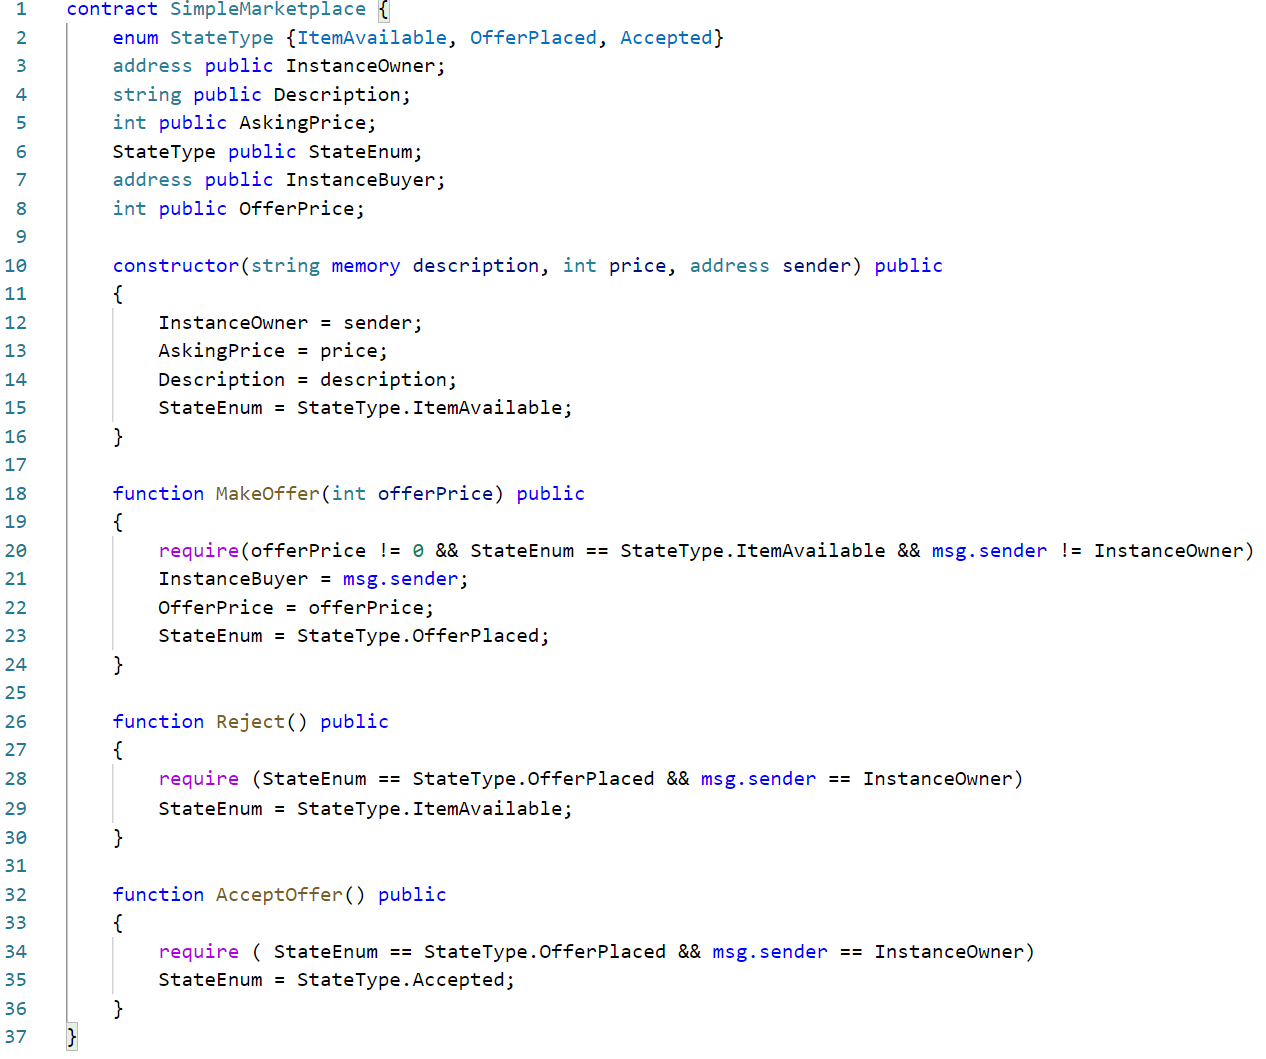
\includegraphics[width=\textwidth]{figs/simple-marketplace.png}}
    \caption{Contrato Inteligente \texttt{SimpleMarketplace} en Solidity}
    \label{fig:solidity-example}
\end{figure}

\section{Enabledness-Preserving Abstractions}


Una EPA es un Labeled Transition System (LTS) finito que busca abstraer el comportamiento de un contrato inteligente agrupando los estados del contrato en base a cuáles de sus metodos están habilitados \cite{de-caso-epa}.
Las transiciones en estos LTS representan el llamado a una función del contrato, indicando cómo un llamado a una función puede transformar el contrato de un estado abstracto a otro.

Comenzando por un ejemplo, en la figura \ref{fig:epa-example} presentamos la EPA del contrato \texttt{Simple\-Marketplace}.
El estado incial, denominado \textbf{A}, está etiquetado \texttt{init} e indica el estado ``vacío'' previo al llamado al constructor del contrato.
Lo que podemos ver es que luego de ejecutar el método constructor se transiciona en la EPA a un único otro estado, al que llamamos \textbf{B}.
Allí, la etiqueta \texttt{\_MakeOffer} indica que \textcolor{orange}{\texttt{MakeOffer}} es el único método que se encuentra habilitado en \textbf{B}.
La única transición desde \textbf{B}, etiquetada \textcolor{orange}{\texttt{MakeOffer}}, indica lo que ocurre cuando se ejecuta ese método desde ese estado. Como vemos, seguir esa transición nos traslada  al estado \textbf{C}, que es un estado del contrato en el que solamente \textcolor{orange}{\texttt{AcceptOffer}} y \textcolor{orange}{\texttt{Reject}} se encuentran habilitados.
Luego, desde el estado \textbf{C} podemos ejecutar cualquiera de los dos métodos; la transición por \textcolor{orange}{\texttt{Reject}} nos llevará de vuelta al estado \textbf{B} y la transición por \textcolor{orange}{\texttt{AcceptOffer}} nos llevará al estado final \textbf{D}.
Este último, etiquetado ``\texttt{vacio}'' indica que ningún método se encuentra habilitado, por lo que representa el fin forzoso de la ejecución.



\begin{figure}
    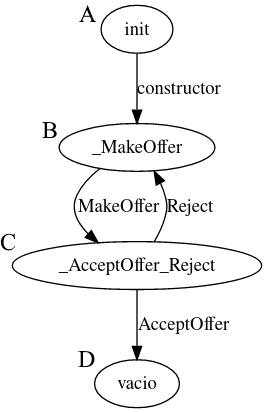
\includegraphics[width=0.3\textwidth]{figs/simple-merketplace-epa.png}
    \caption{EPA de \texttt{SimpleMarketplace}. Las etiquetas en los estados indican los métodos que se encuentran habilitados. Las etiquetas en las transiciones indican el método por el que ocurre la transición.}
    \label{fig:epa-example}
\end{figure}

\section{Modelo Formal}
Dado que trabajaremos sobre el código fuente de un contrato escrito en Solidity, nos interesa formalizar qué aspectos del contrato consideraremos relevantes.
Para obtener una discusión más detallada de estas formalizaciones de los artefactos de código, referirse a De Caso et. al.  \cite{de-caso-epa}.
Asimismo, la abstracción presentada del comportamiento de los contratos inteligentes origina en Godoy et. al. \cite{predicate-abstraction-for-smart-contract-validation}.
En esta sección solamente presentamos una compatibilización de los formalismos para facilitar la discusión de las EPAs más adelante.

Dicho eso, llamaremos \textit{configuraciones} a las posibles combinaciones de las variables de estado del contrato y de la blockchain, y notaremos $C$ al conjunto de todas las posibles configuraciones.

\begin{definition}(Formalización de un contrato inteligente)
    \label{definicion-smart-contract}
    Definimos a un contrato inteligente como la tupla $SC = \langle M, F, R, inv, init \rangle$ donde:

    \begin{itemize}
        \item $M = {m_1, \dots m_n}$ es el conjunto finito de métodos externos definidos en la interfaz del contrato
        \item $F$ es un conjunto de funciones indexadas por $M$. \\
              Para cada $m \in M$, $F_m : C \times \mathds{Z} \rightarrow (C \cup \bot)$ es la implementación del método $m$.
        \item $R$ es un conjunto de precondiciones indexado por $M$.\\
              Para cada $m \in M$, $R_m : C \times \mathds{Z} \rightarrow \{$\textbf{true}, \textbf{false}$\}$ indica si el método $m$ está habilitado para la configuración y parámetros indicados
        \item $inv : C \rightarrow \{$\textbf{true}, \textbf{false}$\}$ indica si una configuración cumple el invariante del contrato
        \item $init : C \rightarrow \{$\textbf{true}, \textbf{false}$\}$ indica si una configuración puede ser resultante de ejecutar el constructor del contrato
    \end{itemize}
\end{definition}

Una particularidad presente en los métodos de los contratos inteligentes es que algunas instrucciones como \textcolor{blue}{\texttt{msg.sender}}, \textcolor{blue}{\texttt{msg.value}}, \textcolor{blue}{\texttt{tx.gasprice}} o \textcolor{blue}{\texttt{tx.origin}}
\footnote{\textcolor{blue}{\texttt{msg.value}} indica cuánto Ether está recibiendo el contrato. \textcolor{blue}{\texttt{tx.gasprice}} indica cuánto Ether se le cobra al remitente por cada unidad de gas (cómputo) utilizada y \textcolor{blue}{\texttt{tx.origin}} se refiere a el usuario humano que haya enviado el mensaje que disparó la ejecución actual.} hacen referencia a variables de la blockchain.
Sin embargo podemos modelar estas variables, junto con los parámetros explícitos como input codificable en $\mathds{Z}$ (los números enteros) sin pérdida de generalidad \cite{de-caso-epa}.
La semántica de un contrato la definimos como el siguiente Labeled Transition System:

\begin{definition}\label{definicion-lts}(Semántica de un contrato inteligente)
    Dado $SC = \langle M, F, R, inv, init \rangle$ un contrato inteligente, su semántica está provista por el LTS concreto $L_c = \langle \sigma , S_c, S_{0c}, \Delta _c \rangle$ que satisfaga:
    \begin{itemize}
        \item $S_c = \{conf | conf \in C \land inv(conf) = \textbf{true}\}$
        \item $S_{0c} = \{conf | conf \in S_c \land init(conf) = \textbf{true}\}$
        \item $\sigma = (F \times \mathds{Z}) \cup \tau$ es el conjunto de todos los posibles llamados a funciones, junto con un elemento $\tau$ que representa un cambio en la blockchain que ocurra de manera independiente al contrato
        \item $\Delta _c \subseteq S_c \times \sigma \times S_c$
        \item $\forall s_1,s_2 \in S_c, m \in M, z \in \mathds{Z} . \\ (s_1,(F_m,z),s_2) \in \Delta _c \iff \bigg( R_m(s_1,z) = \textbf{true} \land   F_m(s_1,z) = s_2 \bigg)$ \\
              $(s_1,\tau,s_2) \in \Delta _c \iff$ un cambio independiente en la blockchain puede llevarnos del estado $s_1$ al estado $s_2$
    \end{itemize}
\end{definition}
Notar que para cualquier contrato, el conjunto $S_c$ de estados de su LTS concreto es infinito.
Esto es porque las configuraciones tienen en cuenta variables de la blockchain externas al contrato.
Incluso para contratos donde las configuraciones de las variables internas es finita, siempre habrá infinitas configuraciones de las variables externas.
\\

A la EPA (es decir, el LTS abstracto) la definimos entonces de la siguiente manera:

\begin{definition}\label{definicion-epa}(Enabledness-Preserving-Abstraction) Dado $SC = \langle M, F, R, inv, init \rangle$ un contrato inteligente y $L_c = \langle \sigma , S_c, S_{0c}, \Delta _c \rangle$ su LTS concreto, entonces el LTS asbtracto $L_A = \langle M \cup \hat{\tau} , 2^M, P_0, \Delta _A \rangle$ es una EPA del contrato y $\alpha : S_c \rightarrow 2^M$ es la función de abstracción, donde se cumple que:
    \begin{itemize}
        \item $2^M$ es el conjunto de partes de $M$
        \item $\forall s \in S_c \: . \:
                  \alpha(s) = \{m | m \in M \land \exists z \in \mathds{Z} . R_m(s,z) = \textbf{true}\}$
        \item $P_0 = \{\alpha(s_0) | s_0 \in S_{0c} \}$
        \item $\forall s_1,s_2 \in S_c, m \in M, z \in \mathds{Z} . \\ (s_1,(F_m,z),s_2) \in \Delta _c \Rightarrow (\alpha(s_1),R_m,\alpha(s_2)) \in \Delta _A$ \\
              $(s_1,\tau,s_2) \in \Delta _c \Rightarrow (\alpha(s_1),\hat{\tau},\alpha(s_2)) \in \Delta _A$
    \end{itemize}
\end{definition}

El conjunto de estados de la \textit{EPA} es $2^M$ (el conjunto de partes de las precondiciones).
La \textit{función de abstracción} de los estados $s_c$ del LTS concreto a los estados abstractos es $\alpha (s_c) = $ ``el conjunto de métodos cuyas precondiciones son satisfechas por $s_c$''.
Una transición en la EPA entre los estados $s$ y $s'$ etiquetada con el método $m$ significa que existen algún estado concreto $s_c$ y un valor de entrada $z$ para los que $\alpha(s_c) = s$ y  $F_m(s,z)=s_c'$ con $\alpha(s_c') = s'$.
Es decir que algún llamado de $m$ a un estado que se abstrae a $s$ nos da de resultado otro estado que se abstrae a $s'$.
Una transición de $s$ a $s'$ etiquetada  con $\hat{\tau}$, la versión abstracta de $\tau$, indica que existe un estado concreto $s_c$ con $\alpha(s_c) = s$ y que puede ocurrir $\alpha (\tau (s_c)) = s'$.
